\documentclass{article}
%\usepackage{showframe}
%\usepackage{pn}
%\usepackage{entcsmacro}
%\usepackage{placeins}

%%%%%%%%%%%%%%%%%%%%%%%%%%%%%%%%%%
%                                %
% package loading and settings   %
%                                %
%%%%%%%%%%%%%%%%%%%%%%%%%%%%%%%%%%

%%%%%%%%%%%%%%%%%%%%%%%%%%%%%%%%%%%%%%%%%%%%%%%%%%%%%% packages

%% encoding and language
\usepackage[T1]{fontenc}		% output font encoding
\usepackage[utf8]{inputenc}		% input encoding
\usepackage[english]{babel}				% language-specific typesetting

%% extending and fixing tex
\usepackage{tabularx}			% advanced arrays
\usepackage{etex}				% extended memory
\usepackage{etoolbox}
\usepackage{xargs,ifthen}		% programming
\usepackage{fixltx2e} 			% fixes stuff in LaTeX
\usepackage{fnpct}				% better footnotes

%% writing algorithms
\usepackage{algorithmic}

%% Drawings
\usepackage{tikz}
	\usetikzlibrary{calc,arrows,matrix,positioning,fit,decorations.markings}

%% typesetting
\usepackage[scale=0.7]{geometry}
\usepackage					% hyperlinks
		[colorlinks,%linkcolor=darkred,citecolor=darkgreen, urlcolor=darkblue,
		bookmarksnumbered=true,bookmarksopen=true,bookmarksdepth=2,
		pdfusetitle=true]
	{hyperref}
\usepackage{multicol}		% mutliple columns
\usepackage{wrapfig}		% text wrapping around figure
\usepackage{graphicx}		% rotation, rescaling etc.
\usepackage{enumitem}		% custom spacing itemize
\setlist[itemize]{topsep=\parskip,itemsep=0pt,leftmargin=\parindent}

%	\setitemize{itemsep=0pt}
%	\setenumerate{itemsep=0pt}
%	\setitemize{leftmargin=\parindent}
%	\setenumerate{leftmargin=\parindent}
%	\setitemize{topsep=\parskip}
\usepackage{xcolor}			% colors

% typography
\usepackage{blindtext}
\usepackage{xspace}			% smart space after text macros
\usepackage{microtype}		% for typography geeks
\usepackage[autostyle = true, english = american, strict = true, autopunct=true]{csquotes}	% quotes
\usepackage{relsize}		% relative sizes in math 
%\usepackage{ellipsis}

% Math symbols, theorems, fonts
%\usepackage[mathb]{mathabx}
\usepackage{mathpazo}			% sets font (comment for standard font)
\usepackage{amssymb}			% AMS symbols
\usepackage{mathtools}			% other math commands (loads AMSmath)
\usepackage{amsthm}
\usepackage{thmtools}			%
%\usepackage{stix}

% linear logic
\usepackage{cmll}			% EB package for LL
\usepackage{stmaryrd}		% for the parr and with

%%%%%%%%%%%%%%%%%%%%%%%%%%%%%%%%%%%%%%%%%%%%%%%%%%%%%%%%%%%%%% settings

\AtBeginDocument{
	%% itemize symbol
	\renewcommand{\labelitemi}{\scalebox{0.8}{$\circ$}}
	%% less hyphenation
	\hyphenpenalty=1000
	\tolerance=400
	\setlength{\parskip}{2pt}
}

%%%% tweaking space for displayed math
%% defaults for reference

%%\abovedisplayskip=12pt plus 3pt minus 9pt
%%\abovedisplayshortskip=0pt plus 3pt
%%\belowdisplayskip=12pt plus 3pt minus 9pt
%%\belowdisplayshortskip=7pt plus 3pt minus 4pt

\abovedisplayskip=8pt plus 2pt minus 6pt
\abovedisplayshortskip=0pt plus 2pt
\belowdisplayskip=8pt plus 2pt minus 6pt
\belowdisplayshortskip=4pt plus 2pt minus 2pt

%% adding a slight space before/after inline math
%%
%% default = 0pt

\mathsurround=1pt


%%%%%%%% hoshino %%%%%%%%%%%%%%%%%% 
\usepackage[all]{xy}
\SelectTips{eu}{10}


\newtheorem{theorem}{Theorem}[section]
%\newtheorem*{theorem*}{Theorem}
\newtheorem{corollary}[theorem]{Corollary}
\newtheorem{lemma}[theorem]{Lemma}
\newtheorem{proposition}[theorem]{Proposition}
\newtheorem{definition}[theorem]{Definition}
\newtheorem{notation}[definition]{Notation}
\newtheorem*{remark}{Remark}
\newtheorem*{notation*}{Notation}
\newtheorem{conjecture}[theorem]{Conjecture}

%%%%%%%%%%%%%%%%%%%%%%%%%%%%%%%%%%
%                                %
%           macros               %
%                                %
%%%%%%%%%%%%%%%%%%%%%%%%%%%%%%%%%%

%% local (this paper)
\newcommand{\quotient}[2]{\catf{#1}\text{\footnotesize$/\!#2$}}
\newcommand{\quotientsmall}[2]{\catf{#1}\text{\scriptsize$/\!#2$}}
\newcommand{\embed}[1]{\funcf E_{\catf #1}}
\newcommand{\embd}[1]{\funcf d_{\catf #1}}
\newcommand{\embt}[1]{\funcf t_{\catf #1}}
\newcommand{\tra}[1]{\mathbf T(\catf #1)}
\newcommand{\dial}[1]{\mathbf D(\catf #1)}
\newcommand{\state}[1]{\mathbf S(\catf #1)}
\newcommand{\eq}{\sim}
\newcommand{\eqQ}{{\normalfont(\ref{eq_Q})}}
\newcommand{\eqS}{{\normalfont(\ref{eq_S})}}
\newcommand{\quo}{\approxident}
\newcommand{\ye}{\approx}
\newcommand{\yl}[1]{\prec_{#1}}
\newcommand{\yr}[1]{\succ_{#1}}

%% monoidal and traced cat
\newcommand{\monp}{\otimes}
\newcommand{\hide}[1]{{\normalfont\textsf{\textbf{H}}^{#1}}}
\newcommand{\defined}{\!\downarrow}
\newcommand{\inv}{^{-1}}
\newcommand{\symm}[2]{\sigma_{#1,#2}}
\newcommand{\Tr}[1]{{\normalfont\textsf{\textbf{Tr}}}^{#1}}		%trace
\newcommand{\unitobj}{\mathbf 1}				% unit object

%% locutions
\newcommand{\locit}[1]{#1}			% not italic
%\newcommand{\locit}[1]\emph{#1}}	% italic
\newcommand{\eg}{\locit{e.g.}~}
\newcommand{\ie}{\locit{i.e.}~}
\newcommand{\via}{\locit{via}~}
\newcommand{\cf}{\locit{cf.}~}
%\renewcommand{\iff}{\locit{iff}~}
\newcommand{\wloss}{\locit{w.l.o.g.}~} 
\newcommand{\vs}{\locit{vs}~}
\newcommand{\resp}{resp.~}
\newcommand{\etc}{\locit{etc.}\xspace}
\newcommand{\etal}{\locit{et al.}\xspace}

\newcommand{\incise}[1]{---\,#1\,---}
\newcommand{\halfincise}[1]{---\,#1}

%% fonts
\newcommand{\funcf}[1]{\textit{\textsf{#1}}}
\newcommand{\catf}[1]{\mathbb{#1}}

%% text macros
\newcommand{\modulo}{\emph{modulo}\xspace}
\newcommand{\cut}{{\tt cut}\xspace}
\newcommand{\GoI}{{\sc GoI}\xspace}
\newcommand{\GofI}{geometry of interaction\xspace}
\newcommand{\Lcalc}{{\hbox{$\lambda$-cal}culus}\xspace}
\newcommand{\Lterm}{\hbox{$\lambda$-term}\xspace}
\newcommand{\Lterms}{$\lambda$-terms\xspace}
\newcommand{\bred}{\hbox{$\beta$-re}duction\xspace}
\newcommand{\systF}{{\sc System~F}\xspace}
\newcommand{\mells}{MELL\textsubscript{2}\xspace}
\newcommand{\mellp}{MELL\textsubscript{p}\xspace}
\newcommand{\MGU}{MGU\xspace}

%% general math
\newcommand{\ZZ}{\mathbb Z}		% relative integers
\newcommand{\NN}{\mathbb N}		% integers
\newcommand{\RR}{\mathbb R}		% reals
\newcommand{\CC}{\mathbb C}		% complex
\newcommand{\sequ}[1]{\vec{#1}}			% notation for sequences
\newcommand{\norm}[1]{\|#1\|}
\newcommand{\powerset}{\mathcal P}
\newcommand{\adj}[1]{#1^\dagger}				% ajoint
\DeclareMathOperator{\card}{Card}				% cardinal
\newcommand{\extlist}[2]{#1,\,\dots\,,#2}					% list/sequence in extension
\newcommand{\extinflist}[1]{#1,\,\dots}						% list/sequence in extension
\newcommandx{\extset}[3][1=]{#1\{#2,\,\dots\,,#3#1\}}		% set in extension
\newcommand{\extinfset}[1]{\left\{\,#1,\,\dots\,\right\}}		% set in extension
\newcommandx{\set}[3][1=]{#1\{\:#2 \ #1|\ #3\:#1\}}		% set in comprehension
\newcommand{\Id}{\mbox{Id}}										% identity
\newcommand{\void}{\varnothing}									% emptyset
%\newcommand{\empty}{\varnothing}								% emptyset

%% category theory
\newcommand{\sq}{\textbf{\tt;}}									% sequential composition
\newcommand{\morph}[3]{#1:#2\rightarrow #3}		% morphism
\newcommand{\morphc}[4]{#1:#2\rightarrow_{\catf #4} #3}		% morphism
\newcommand{\iso}{\xrightarrow[]{\,_\sim}}						% isomorphism arrow
\newcommand{\isom}[3]{#1\,:\,#2\isom #3}	% morphism
\newcommand{\retr}[2]{\,:\,#1\,\lhd\, #2}		% retraction

%% partial equality
\newcommand{\rightharpoonupeq}{\mathrel{%
\resizebox{\widthof{$=$}}{\height}{%
\raise.22ex\hbox{$\rightharpoonup $}%
\setbox0=\hbox{$\relbar\mkern-9.1mu\relbar$}%
\kern -.98\wd0 \lower.23ex\box0}}}%

\newcommand{\leftharpoonupeq}{\mathrel{%
\resizebox{\widthof{$=$}}{\height}{%
\raise.22ex\hbox{$\leftharpoonup $}%
\setbox0=\hbox{$\relbar\mkern-9.1mu\relbar$}%
\kern -.98\wd0 \lower.22ex\box0}}}%

\newcommand{\leftrightharpooneq}{\mathrel{%
\resizebox{\widthof{$=$}}{\height}{%
\lower.02ex\hbox{$\leftrightharpoons$}%
\setbox0=\hbox{}%
\kern -.98\wd0 \raise.22ex\box0}}}%

\newcommand{\peqr}{\rightharpoonupeq}
\newcommand{\peql}{\leftharpoonupeq}
\newcommand{\peq}{\leftrightharpooneq}

%% triple simeq

\newcommand*{\approxident}{%
  \mathrel{\vcenter{\offinterlineskip
  \hbox{$\sim$}\vskip-.35ex\hbox{$\sim$}\vskip-.35ex\hbox{$\sim$}}}}

%\makeatletter
%\providecommand*{\approxident}{%
%  \mathrel{%
%    \mathpalette\@approxident\sim
%  }%
%}   
%\newcommand*{\@approxident}[2]{%
%  \sbox0{$#1\vcenter{}$}%
%  \sbox2{$\m@th#1\equiv$}%
%  \dimen2=\dimexpr\ht2 - \ht0\relax
%  \sbox4{$\m@th#1\sim$}%
%  \dimen4=\dimexpr\ht4 - \ht0\relax
%  \dimen0=\dimexpr
%    -\ht4 - \dp4 %
%    + \dimen2 %
%  \relax
%  \vcenter{\offinterlineskip
%    \copy4 %
%    \kern\dimen0 %
%    \copy4 %
%    \kern\dimen0 %
%    \copy4 %
%    \ifdim\dp4=\z@
%      \kern\dimexpr -\ht0 + \dimen4\relax
%    \fi
%  }%   
%}      
%\makeatother

%%%%%% hoshino %%%%%%%%
\newcommand{\SMC}{\mathbf{SMC}}
\newcommand{\TSMC}{\mathbf{TSMC}}
\newcommand{\SMCiso}{\mathbf{SMC}_{\mathrm{iso}}}
\newcommand{\TSMCiso}{\mathbf{TSMC}_{\mathrm{iso}}}
\newcommand{\Pfn}{\mathbb{P}}
\newcommand{\U}{\mathbf{U}}
\newcommand{\F}{\mathbf{F}}



\begin{document}

%\hypersetup{bookmarksopen=true,bookmarksdepth=2}

%%%%% TITLE
%\def\lastname{Bagnol}

\title{A Free Trace Construction and the Embedding Problem}

\author{Marc Bagnol, Naohiko Hoshino, Masahito Hasegawa, Léo Stefanesco}

\maketitle

\begin{abstract}
	The notion of trace in a monoidal category allows
to give a category-theoretic account of the notion of feedback, and instances of
it can be found in linear algebra, topology, knot theory and proof theory. An extension to the 
partially defined case has also more recently been studied.

In this article, an explicit construction of the free trace in a symmetric monoidal category is presented,
defined by considering morphisms equiped with a form of private state space and taking a 
suitable quotient.
Conditions for this construction to yield an embedding of the original category into the free traced
one are discussed and called the embedding problem. 
This relates to the notion of partially traced category as it is already known that a symmetric
monoidal category can be equiped with a partial trace if and only if it can be embedded into a
totally traced one.

Examples are considered, using the free construction to determine the free trace on
some standard symmetric monoidal categories, and showing that some classic example of traces are not free.
The extension of the construction to the braided case appears to be straightforward and is sketched in
the end of the article.

\end{abstract}

\addcontentsline{toc}{section}{Introduction}
\section*{Introduction}
\begin{itemize}
	\item Present the notion of trace
	\item Mention the story of partial trace and the embedding problem (Scott, Selinger)
	\item Outline paper
\end{itemize}



\section{Traced and partially traced categories}
\begin{itemize}
	\item Brief technical account of trace, axioms, diagramatic language etc. example
	\item Partial case as a slight variation. example
\end{itemize}



\section{The dialect construction and hiding}
%\begin{itemize}
%	\item definition of the dialect construction
%	\item hiding operation, free pseudo-trace
%\end{itemize}


The first step of the construction is, starting with a SMC, to equip morphisms with a notion of
\emph{state} or \emph{private space}. As the name suggests, when composing two such morphisms
the private parts will avoid each other and not interact. The basic idea here is that any interface
in the private space is unerstood as \emph{virtually} traced and subjected to the trace equations.
We detail and formalize this in the following definition.

\begin{definition}[state pseudo-category]
	Let $\catf C$ be a symmetric monoidal category. Define $\state C$ the \emph{state 
	pseudo\footnotemark-category}
	over $\catf C$ as:
	\begin{itemize}
		\item The objects of $\state C$ are those of $\catf C$.
		\item A morphism from $A$ to $B$ in $\state C$ is a pair $(f,U)$,
		where $U$ is an object of $\catf C$ and $\morph f{A\monp U}{B\monp U}$ is a morphism of 
		$\catf C$.
		\item The identity on $A$ is defined as the pair $(\Id_A, \unitobj)$.
		\item Composition of morphisms $\morph{(f,U)}{A}{B}$ and $\morph{(g,V)}{B}{C}$ is defined by
		$$(f,U)\sq(g,V)=\big(\:
		( f\monp V)\sq(B\monp \symm UV)\sq(g\monp U)\sq(C\monp\symm VU)
		\:,\,U\monp V\,\big)$$
		\FIGURE{composition}
	\end{itemize}
\end{definition}
\footnotetext{Composition does not necessarily satisfy associativity yet.}

Unless $\catf C$ is strict, $\state C$ will not be a proper category in general: if we have objects
such that $U\monp (V\monp W)\neq (U\monp V)\monp W$ then morphisms
$(f,U) \sq \big((g,V) \sq (h,W)\big)$ and $\big((f,U) \sq (g,V)\big) \sq (h,W)$ cannot be equal.
However, everything becomes  perfectly fine if we look at state-equiped morphisms 
\emph{up to sliding isomorphisms}, one of the trace equations. This leads to the definition of the
\emph{dialect category}, the name dialect paying tribute to a similarly named construction introduced
by J.-Y. Girard in his work on geometry of interaction~\cite{girard95}.

\begin{definition}[dialect category]
	The \emph{dialect category} $\dial C$ over $\catf C$ is defined by quotienting morphisms of
	$\state C$ by the following equivalence relation, which we call \emph{sliding equivalence}:
		$$\big(\,f\sq(B\monp\phi)\,,\,U\,\big)\eq \big(\,(B\monp\phi)\sq f\,,\,V\,\big) \text{ \ for any 
		$\catf C\!$-isomorphism\footnotemark $\morph\phi VU$ and 
		$\morph f{A\monp U}{B\monp V}$}
		$$
		\FIGURE{sliding in state category}
		\footnotetext{One could choose to allow sliding of \emph{any} morphisms here.
		But in the presence of yanking one can recover the full case where $\phi$ is any
		morphism from the isomorphism case~\cite{jsv96}. Moreover sliding only isomorphisms is 
		enough to make $\dial C$ a category and isomorphisms are more convenient to manipulate.
		}
\end{definition}

Once this definition is set up, it is an easy exercise to check that the composition operation
becomes associative in $\dial C$ and that the $(\Id_A, \unitobj)$ are neutral.

\begin{proposition}
	After quotienting, $\dial C$ is indeed a category.
\end{proposition}

\begin{proposition}
	There is a functorial embedding $\embd C$ of $\catf C$ into $\dial C$ defined as the identity on
	objects and $\embd C (f)=(f\monp \Id_{\unitobj}, \unitobj)$ on morphisms.
\end{proposition}

\begin{proof}
	The fact that $\embd C(f\sq g)=\embd C(f) \sq \embd C(g)$ follows readily from the structure
	equations involving $\unitobj$. Then, if $\embd C(f) \eq \embd C(g)$, this means that there
	exist $\morph{f'}{A\monp \unitobj}{B\monp \unitobj}$, 
	$\morph{g'}{A\monp \unitobj}{B\monp \unitobj}$ and an isomorphism $\morph\phi\unitobj\unitobj$
	such that $f\monp\Id_\unitobj=f'\sq (\Id_B\monp\phi)$ and 
	$g\monp\Id_\unitobj=(\Id_A\monp\phi)\sq g'$. General properties of morphisms from $\unitobj$ to
	$\unitobj$ in monoidal categories imply that, for instance, $(\Id_A\monp\phi)\sq g'=g'\sq (\Id_B\monp\phi)$,
	so that $f'=g'$ and eventually $f=g$.
\end{proof}

Moreover the monoidal structure of $\catf C$ can be lifted to $\dial C$.

\begin{proposition}[monoidal structure]
	We can define the following monoidal structure on $\dial C$:
	\begin{itemize}
		\item The unit object $\unitobj$ is the one from $\catf C$.
		\item The bifunctor $\monp$ is defined the same way on objects and as follows on morphisms:
		$$(f,U)\monp(g,V)=(A\monp \symm CU\monp V)\sq(f\monp g)\sq(B\monp \symm UD\monp V)
		$$
		(with $\morph f{A\monp V}{B\monp V}$ and $\morph g{C\monp V}{D\monp V}$)
		\item All the structure isomorphisms are obtained \via the embedding $\embd C$, \eg the
		symmetries are defined as $(\symm AB, \unitobj)$.
	\end{itemize}
\end{proposition}

\begin{proof}
	We first have to make sure that the new $\monp$ is well-defined, \ie that it is compatible with
	$\eq$, explicitely: whenever $(f,U)\eq(g,V)$ then for any $(h,W)$ we have 
	$\big((h,W)\monp(f,U)\big)\eq\big((h,W)\monp(g,V)\big)$ and 
	$\big((f,U)\monp(h,W)\big)\eq\big((g,V)\monp(h,W)\big)$ which follows immediately after carefully
	unfolding the definitions.

	Because we defined the structure isomorphisms using a functorial embedding, all the needed
	structure equations carry over to $\dial C$. The only thing remaining to check is whether
	the families of structure isomorphisms thus defined are still natural.
	Let us look at the case of symmetries to see what type of computation we are dealing with. The
	other cases are similar.
	
	\FIGURE{graphical computation}
\end{proof}

Now that we have this general context to work in, we can already remark something interesting:
if we have a morphism $\morph{(f,V)}{A\monp U}{B\monp U}$ in $\dial C$ (that is, a morphism
$\morph f {A\monp U\monp V}{A\monp U\monp V}$ in $\catf C$) there is a natural operation that can be
performed which resembles taking a trace, at least at the level of interfaces: one can push $U$
to the private part of $f$, making it a morphism from $A$ to $B$ in $\dial C$.

\begin{definition}[Hiding]
	Given a morphism $\morph{(f,V)}{A\monp U}{B\monp U}$ of $\dial C$, define 
	$$\hide U[V,f]=(f,U\monp V)$$
	We call this operation \emph{hiding $U$}.
\end{definition}

This operation not only shares the action on interfaces of a trace, it also has most of the required
properties of traces. Most notably since we defined $\dial C$ \via making sliding equations into equalities,
it satisfies sliding. Even more than that, the pseudo-trace structure obtained is the free one.

\begin{theorem}[free pseudo trace]
	The hiding operation $\hide{}[\cdot]$ defines a pseudo-trace (\ie a trace minus yanking)
	in $\dial C$.
	Moreover, $\dial C$ satisfies the following universal property: for any pseudo-traced
	category $\catf D$ and monoidal functor $\morph F{\catf C}{\catf D}$ we have that $F$
	factors uniquely as 
	\begin{center}
	$\funcf F=\funcf G\circ \embd C$ \qquad\qquad
	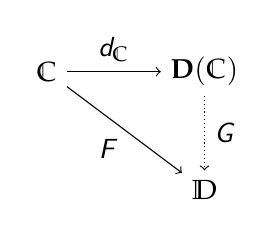
\begin{tikzpicture}[baseline=-5ex]
		\node (c) at (0,0) {$\catf C$};
		\node (tc) at (2,0) {$\dial C$};
		\node (d) at (2,-1.5) {$\catf D$};
		\draw[->] (c) to node [above] {$\embd C$} (tc);
		\draw[->] (c) to node [below left] {$\funcf F$} (d);
		\draw[->,densely dotted] (tc) to node [right] {$\funcf G$} (d);
	\end{tikzpicture}
\end{center}
	with $G$ a pseudo-traced functor.
\end{theorem}

\begin{proof}
\TODO{More detailed proof than in my short note.}
%	Set $G(f,U)=\Tr{\funcf FU}[\funcf F f]$ (this is well defined because $\Tr{}$ satisfies sliding)
%	with structure maps being those of $F$.
%	It factors $F$ because of vanishing and $\funcf F\unitobj\simeq\unitobj$, and is indeed a
%	pseudo-traced functor because we defined it using $\Tr{}$.
%	
%	An easy computation gives the unicity property.
\end{proof}

%\begin{remark}
%	This universal property implies that $\dial \cdot$ is a functor.
%\end{remark}





\section{Yanking and free trace}
\begin{itemize}
	\item adding the missing equation via a further quotient
	\item free trace
\end{itemize}


%We now want to enforce the yanking equation on $\hide{}[\cdot]$ in $\dial C$. To do so, we follow 
%the same approach as
%before and further quotient $\dial C$.

%\begin{definition}[trace category]
%	Define the following relation on $\state C$ morphisms:
%	$$\big(\,(f\monp V)\sq(B\monp\symm VV)\sq(g\monp V)\,,\, U\monp V\,\big)
%	\yr V (f\sq g\,,\,U) $$
%	and set $f\yl{}g=g\yr{}f$. These are then lifted to $\dial C$ morphisms by saying that two
%	equivalence class are related whenever they contain two related elements.
%	
%	We obtain two equivalence relations:
%	\begin{itemize}
%		\item In $\dial C$, the transitive closure of $\yr{}\cup\yl{}$, which we write $\ye$.
%		\item In $\state C$, the transitive closure of $\eq\cup\yr{}\cup\yl{}$, which we write $\quo$.
%	\end{itemize}
%	The \emph{trace category} over $\catf C$ is defined as $\tra C=\quotient{\dial C}{\ye}
%	=\quotient{\state C}{\quo}$,
%	that is the category $\dial C$ where morphisms are further equated by $\ye$ or equivalently
%	the pseudo-category $\state C$ with morphisms equated by $\quo$.
%\end{definition}

%\begin{proposition}
%	The above defined $\tra C$ is indeed a category and
%	the symmetric monoidal structure of $\dial C$ lifts to $\tra C$.
%\end{proposition}

%\begin{proof}
%	Amounts to showing that $\yr{}$ is a \enquote{monoidal congruence}, graphical computations
%	make this fairly straightforward.
%\end{proof}

%\begin{proposition}
%	There is a monoidal functor $\embt C$ from $C$ to $\tra C$, defined as
%	$\embt C(f)=(f,\unitobj)$.
%\end{proposition}

%\begin{remark}
%	As we observed, this is not necessarily an embedding.
%\end{remark}

%\begin{theorem}
%	The hiding operation $\hide{}[\cdot]$ lifts to $\tra C$ and makes it a traced category.
%	
%	Moreover, $\tra C$ satisfies the following universal property: for any traced
%	category $\catf D$ and monoidal functor $\morph F{\catf C}{\catf D}$ we have that $F$
%	factors uniquely as 
%	\begin{center}
%	$\funcf F=\funcf G\circ \embt C$ \qquad\qquad
%	\begin{tikzpicture}[baseline=-5ex]
%		\node (c) at (0,0) {$\catf C$};
%		\node (tc) at (2,0) {$\tra C$};
%		\node (d) at (2,-1.5) {$\catf D$};
%		\draw[->] (c) to node [above] {$\embt C$} (tc);
%		\draw[->] (c) to node [below left] {$\funcf F$} (d);
%		\draw[->,densely dotted] (tc) to node [right] {$\funcf G$} (d);
%	\end{tikzpicture}
%	\end{center}
%	with $G$ a traced functor.
%\end{theorem}

%\begin{proof}
%	Same as in the previous section: define $G(f,U)=\Tr{\funcf FU}[\funcf F f]$.
%\end{proof}


%\begin{remark}
%	As before, this implies that $\tra\cdot$ is a functor. We could probably define in the same 
%	spirit an operation that takes a pseudo-traced category as an input (not necessarily the
%	result of applying $\dial\cdot$) and freely makes it a traced category.
%\end{remark}


%%% TeX-master: "MAIN" %% Please do not remove this line (hoshino)

\section{\(2\)-adjunction}
\label{2-adjunction}

Let \(\SMCiso\) be the \(2\)-category of symmetric monoidal categories,
strong symmetric monoidal functors and monoidal natural
isomorphisms; and let \(\TSMCiso\) be the \(2\)-category of traced
symmetric monoidal categories, traced symmetric monoidal functors and
monoidal natural isomorphisms. We prove that
\(\U\) is a right \(2\)-adjoint. To see this, we show that
\begin{equation*}
  \TSMCiso(\F\catf{A},\catf{B}) \xrightarrow{\U}
  \TSMCiso(\U\F\catf{A},\U\catf{B}) \xrightarrow{(-) \circ \embed{A}}
  \SMCiso(\catf{A},\U(\catf{\catf{B}})).
\end{equation*}
is an isomorphism.

For a symmetric monoidal functor \(F \colon \catf{A} \to \U(\catf{B})\),
we define a traced symmetric monoidal functor \(F^{\vee} \colon \F\catf{A} \to \catf{B}\)
as follows:
\begin{align*}
  F^{\vee}(X) &= F, \\
  F^{\vee}((f,U) \colon X \to Y)
  &= \Tr{FU}_{FX,FY}((m_{Y,U}^{F})^{-1} \circ Ff \circ m_{X,U}), \\
  n^{F^{\vee}} &= n^{F} \colon I \to F, \\
  m^{F^{\vee}}_{X,Y} &= m^{F}_{X,Y} \colon FX \otimes FY \to F(X \otimes Y).
\end{align*}
For a monoidal natural isomorphism \(\alpha \colon F \to G\), we
define a monoidal natural isomorphism \(\alpha^{\vee} \colon F \to G\)
to be \(\alpha\).

Below, we check that \((-)^{\vee}\) is a functor and \(\alpha^{\vee}\)
is a monoidal natural isomorphism.
We first check that \(F^{\vee}\) is a functor. For \(X \in \catf{A}\),
\begin{align*}
  F^{\vee}(\Id_{X \otimes I},I)
  &= \Tr{FI}_{FX,FX}(\Id_{FX \otimes FI}) \\
  &= \Tr{I}_{FX,FX}(\Id_{FX \otimes I}) \\
  &= \Id_{FX}.
\end{align*}
For \(\F\catf{A}\)-morphisms \((f,U) \colon X \to Y\) and \((g,V)
\colon Y \to Z\), we denote \((m_{Y,U}^{F})^{-1} \circ Ff \circ
m_{X,U}\) by \(f'\) and \((m_{Z,V}^{F})^{-1} \circ Fg \circ m_{Y,V}\)
by \(g'\). Then
\begin{align*}
  F^{\vee}(g,V) \circ F^{\vee}(f,U)
  &= \Tr{FV}_{FY,FZ}(g') \circ \Tr{FU}_{FX,FY}(f') \\
  &= \Tr{FU \otimes FV}_{FX,FZ}(FY \otimes \symm{FV}{FU}) \circ
  (g' \otimes FU) \circ (FY \otimes \symm{FU}{FV}) \circ (f' \otimes FV)) \\
  &= \Tr{FU \otimes FV}_{FX,FZ}(((m_{Z,V}^{F})^{-1} \otimes FU) \circ
  (m_{Z \otimes V,U}^{F})^{-1} \circ
  Fh \circ m_{X \otimes U,V}^{F} \circ (m_{X,U}^{F} \otimes FV)) \\
  &= \Tr{F(U \otimes V)}_{FX,FZ}((m_{Z,U \otimes V}^{F})^{-1} \circ
  Fh \circ m_{X, U \otimes V}^{F}) \\
  &= F^{\vee}((g,V) \circ (f,U))
\end{align*}
where \(h \colon X \otimes U \otimes V \to Z \otimes U \otimes V\) is given by
\begin{equation*}
  (Z \otimes \symm{V}{U}) \circ (g \otimes U) \circ (Y \otimes \symm{U}{V})
  \circ (f \otimes V).
\end{equation*}
We next check naturality of \(m^{F^{\vee}}_{X,Y}\). For
\(\F\catf{A}\)-morphisms \((f,U) \colon X \to Z\) and \((g,V) \colon Y
\to W\), we denote \((m^{F}_{Z,U})^{-1} \circ Ff \circ m^{F}_{X,U}\) by
\(f'\) and \((m_{W,V}^{F})^{-1} \circ Fg \circ m^{F}_{Y,V}\) by \(g'\). Then
\begin{align*}
  &m^{F}_{Z,W} \circ (F^{\vee}(f,U) \otimes F^{\vee}(g,V)) \\
  &= \Tr{FU \otimes FV}_{FX \otimes FY,F(Z \otimes W)}
  ((m^{F}_{Z,W} \otimes FU \otimes FV) \circ
  (FZ \otimes \symm{FU}{FW} \otimes FV) \circ
  (Ff' \otimes Fg') \circ
  (FX \otimes \symm{FU}{FY} \otimes FV)) \\
  &= \Tr{F(U \otimes V)}_{FX \otimes FY,F(Z \otimes W)}
  ((m_{Z \otimes W, U \otimes V}^{F})^{-1} \circ
  Fh \circ
  m_{X \otimes Y, U \otimes V}^{F} \circ
  (m_{X,Y}^{F} \otimes F(U \otimes V))) \\
  &= F^{\vee}((f,U) \otimes (g,V)) \circ m^{F}_{X,Y}
\end{align*}
where \(h \colon X \otimes Y \otimes U \otimes V \to Z \otimes W \otimes U \otimes V\)
is given by
\begin{equation*}
  h = (Z \otimes \symm{U}{W} \otimes V) \circ (f \otimes g) \circ
  (X \otimes \symm{Y}{U} \otimes V).
\end{equation*}
Preservation of trace operators by \(F^{\vee}\) follows from Vanishing
II. Coherence conditions for \(m^{F^{\vee}}\) follows from those for
\(m^{F}\). Lastly, we check that \(\alpha^{\vee}\) is a monoidal
natural isomorphism. Since coherence conditions for \(\alpha^{\vee}\)
follow from those for \(\alpha\), we only check naturality of
\(\alpha^{\vee}\). For a \(\F\catf{A}\)-morphism \((f,U) \colon X \to
Y\),
\begin{align*}
  \alpha_{Y} \circ F^{\vee}(f,U)
  &= \Tr{FU}_{FX,GY}((\alpha_{Y} \otimes FU) \circ (m^{F}_{Y,U})^{-1} \circ Ff \circ m^{F}_{X,U}) \\
  &= \Tr{GU}_{FX,GY}((\alpha_{Y} \otimes \alpha_{U}) \circ (m^{F}_{Y,U})^{-1} \circ Ff \circ m^{F}_{X,U}
  \circ (FX \otimes \alpha^{-1}_{U})) \\
  &= \Tr{GU}_{FX,GY}((m^{G}_{Y,U})^{-1} \circ Gf \circ m^{G}_{X,U}
  \circ (\alpha_{X} \otimes GU)) \\
  &= G^{\vee} (f,U) \circ \alpha_{X}.
\end{align*}

\begin{proposition}
  \((-)^{\vee}\) is the inverse of \(\U(-) \circ \embed{A}\).
\end{proposition}
\begin{proof}
  For \(F \colon \catf{A} \to \U\catf{B}\),
  \begin{align*}
    (\U (F^{\vee}) \circ \embed{A})(f \colon X \to Y)
    &= \Tr{FI}_{FX,FY} ((m^{F}_{Y,I})^{-1} \circ F(f \otimes I) \circ m^{F}_{X,I}) \\
    &= Ff.
  \end{align*}
  For \(G \colon \F\catf{A} \to \catf{B}\),
  \begin{align*}
    ((\U G) \circ \embed{A})^{\vee}((f,U) \colon X \to Y)
    &= \Tr{GU}_{GX,GY}((m^{G}_{Y,U})^{-1} \circ G(f \otimes I,I) \circ m^{G}_{X,U}) \\
    &= G(\hide{U}(f \otimes I,I)) \\
    &= G(f,U).
  \end{align*}
  It is straightforward to check
  \(\U (\alpha^{\vee}) \circ \embed{A} = \alpha\)
  for any \(\alpha \colon F \Rightarrow G \colon \catf{A} \to \U\catf{B}\)
  and \(((\U \beta) \circ \embed{A})^{\vee} = \beta\) 
  for any \(\beta \colon F \Rightarrow G \colon \F\catf{A} \to \catf{B}\).
\end{proof}

\paragraph{Failure of a Generalization}

The forgetful \(2\)-functor \(\U' \colon \TSMC \to \SMC\) is no longer
a right \(2\)-adjunction where \(\TSMC\) is the \(2\)-category of traced
symmetric monoidal categories, traced symmetric monoidal functors and
\emph{monoidal natural transformations}, and \(\SMC\) is the
\(2\)-category of symmetric monoidal categories, strong symmetric
monoidal functors and \emph{monoidal natural transformations}.

We suppose that \(\U'\) has a left \(2\)-adjunction \(\F'\) and derive
a contradiction. If \(\F'\) is left \(2\)-adjoint to \(\U'\), then
\(\F'\catf{A}\) is isomorphic to \(\F\catf{A}\) for any traced
symmetric monoidal categories \(\catf{A}\). Therefore,
\begin{equation*}
  \TSMC(\F\Pfn,\F\Pfn) \xrightarrow{\U}
  \TSMC(\U'\F\Pfn,\U'\F\Pfn) \xrightarrow{(-) \circ \embed{\Pfn}}
  \SMC(\Pfn,\U'\F\Pfn)
\end{equation*}
is an isomorphism where \(\Pfn\) is the category of sets and partial
functions regarded as a symmetric monoidal category by taking the
disjoint sum of sets as its monoidal product. Let \(N \colon \Pfn \to
\F(\Pfn)\) be a strong symmetric monoidal functor given by \(N(X) =
\emptyset\). For a set \(X\), we define \(z_{X} \colon X \to
\emptyset\) to be the empty partial function. Because \(z_{X}\) is a
monoidal natural transformation from \(\embed{\Pfn}\) to \(N\) and
\(\U(-) \circ \embed{\Pfn}\) is an isomorphism, \(z_{X}\) is also a
monoidal natural transformation from \(\Id_{\F\Pfn}\) to \(N^{\vee}\).
By the definition of \((-)^{\vee}\), we see that \(N^{\vee}(f \colon X
\to Y)\) is equal to the empty partial function from \(X\) to \(Y\)
for any partial function \(f \colon X \to Y\). By naturality of
\(z_{X}\), the following diagram commutes:
\begin{equation*}
  \xymatrix{
    1 \ar[r]^{\Tr{\NN}_{1,1}(f)} \ar[d]_{z_{1}} &
    1 \ar[d]^{z_{1}} \\
    \emptyset \ar@{=}[r] &
    \emptyset
  }
\end{equation*}
where \(f \colon \{\ast\} + \NN \to \{\ast\} + \NN\) is given by
\begin{align*}
  f(\ast) &= 0, \\
  f(n) &= n+1.
\end{align*}
However, we have \(z_{1} \circ \Tr{\NN}_{1,1}(f) \neq z_{1}\) as we observed in (...).


\section{The embedding problem and partial traces}
\begin{itemize}
	\item embedding problem and the free trace
	\item more details on failed solutions, counterexaples for the embeding problem
	\item Hassei's note point of view: IY, IYe etc.
	\item partial results and conjecture
\end{itemize}


%This leads us to a reformulation of the \enquote{embedding problem}:

%\begin{theorem}[the embedding problem]
%	A monoidal category $\catf C$ can be embedded into a traced one if and only if the functor
%	$\embt C$ is an embedding (or, more explicitely: $f=g\iff (f,\unitobj)\ye(g,\unitobj)$).
%\end{theorem}

%Also, this is related to partial traces since we know \cite{mss12,bagnol15a} that symmetric
%monoidal category can be equipped with a partial trace if and only if it can be embedded into
%a traced category.
%By the way, we can see that the partial trace obtained that way the \enquote{smallest}
%possible (in the sense: the least defined).

%\begin{proposition}
%	If we have two embeddings $E_1,E_2$ of $\catf C$ into traced categories $\catf D_1,\catf D_2$,
%	such that there is a traced functor $G$ making the following diagram commute
%	\begin{center}
%	\begin{tikzpicture}[baseline=-5ex]
%		\node (c) at (0,0) {$\catf C$};
%		\node (tc) at (2,0) {$\catf D_1$};
%		\node (d) at (2,-1.5) {$\catf D_2$};
%		\draw[->] (c) to node [above] {$\funcf E_1$} (tc);
%		\draw[->] (c) to node [below left] {$\funcf E_2$} (d);
%		\draw[->] (tc) to node [right] {$\funcf G$} (d);
%	\end{tikzpicture}
%	\end{center}
%	then the associated partial traces $\Tr{}_1,\Tr{}_2$ on $\catf C$ are related as follows:
%	the domain $D$ of $\Tr{}_1$ is contained in that of $\Tr{}_2$ and the two traces agree on $D$.
%\end{proposition}

%Indeed, the universal property of the previous section ensures that the domain of the partial trace
%induced by $\embt C$ (when it is an embedding) is the smallest possible for a partial trace.

%\subsection*{Embedding condition}

%What we still need to understand is under which conditions on $\catf C$ the functore $\embt C$ is an
%embedding. Ideally we are looking for a condition that is really formulated in the language of
%$\catf C$ and synthetic. We saw that several attempts \enquote{Scott's condition}, 
%\enquote{Selinger's condition} turned out to be necessary but not sufficient.

%For this specific question, I think it will be easier to work in $\state C$, where equality is plain
%equality. This becomes a problem of understanding what can happen when we have a chain of 
%$\eq,\yr{},\yl{}$.

%It is fair to say that we do not really know for now what would a sufficient condition be like.
%So to get started, I think we can explore the properties of chains of $\eq,\yr{},\yl{}$ to
%understand better how they rewrite, what properties they always have \etc
%this could help us pinpoint exactly what is missing to get an embedding, or at least make it easier
%to check whether a new proposed condition is sufficient.

%I'll list some basic results. (I have proof sketches for non-conjecture ones)

%\begin{lemma}[$\eq$ before $\yr{}$]
%	Whenever we have $f\yr{}g\eq g'$ ($f,g,g'$ are in $\state C$) then there exists a $f'$ such that
%	$f\eq f'\yr{}g$. Similarly, $g\eq g'\yl{}f$ implies $g\yl{}f'\eq f$.
%\end{lemma}

%This means that a chain of equivalences $f\quo g$ can always be rewritten as a sequence of blocks of the
%form $h\yl{}^*g\eq g'\yr{}^* f$, where $\yl{}^*$ and $\yr{}^*$ are the transitive closures of 
%$\yl{}$ and $\yr{}$.

%\begin{conjecture}
%	...
%\end{conjecture}


%\subsection*{Naohiko's counterexample}

%Something to discuss when I come to Kyoto: in his original note, Naohiko found a counterexample to
%the sufficiency of Selinger condition, which was attributed to the condition not taking sliding into
%account.

%Yet as we discussed there the IYS condition restricted to sliding only isomorphism is not stronger than
%the IY condition.

%There is an alternative way to look at this, based on the way one gets full sliding from sliding only
%symmetries, where the counterexample appears as rather a failure of \emph{confluence}. I'll just
%include handwritten notes for now as graphical calculations take ages to type, and non-graphical
%are hard to read:









\section{Free and non-free traces}
\begin{itemize}
	\item applying the construction to concrete examples
	\item building the free trace of ... (sets?)
	\item a non-free trace (eg. standard trace on set?)
\end{itemize}


\section{Building the Free Trace of Monoidal Categories with Coproducts}

\subsection{Preservation of Coproducts}

Generally, it is not easy to see how $\tra{A}$ looks like. Below, we
specify our target to symmetric monoidal categories with coproducts.

\begin{lemma}\label{lem:zero-object}
  If $\catf{A}$ has an initial object $0$ such that the canonical morphism
  $0 \to X \otimes 0$ is an isomorphism for any $X \in \catf{A}$,
  then $0$ is an initial object of $\tra{A}$.
\end{lemma}
\begin{proof}
  For any $\tra{A}$-morphism $(f,U) \colon 0 \to X$, we have
  \begin{equation*}
    (f,U) = (0 \otimes U \xrightarrow{\cong}  0 \xrightarrow{\cong} X \otimes U,U)
    = (0 \otimes 0 \xrightarrow{\cong}  0 \xrightarrow{\cong} X \otimes 0,0).
  \end{equation*}
  Hence, $0$ is an initial object of $\tra{A}$.
\end{proof}

\begin{proposition}\label{prop:biproduct}
  If $\catf{A}$ has a zero object $0$ and binary coproducts
  \begin{equation*}
    X \xrightarrow{\iota_{X,Y}} X \oplus Y \xleftarrow{\iota'_{X,Y}} Y
  \end{equation*}
  such that the canonoical morphisms
  \begin{equation*}
    (X \otimes Y) \oplus (X \otimes Z) \xrightarrow{\mathrm{dst}_{X,Y,Z}} X \otimes (Y \oplus Z)
  \end{equation*}
  are isomorphism for all $X,Y,Z \in \catf{A}$, then
  $\tra{A}$ has finite coproducts.
\end{proposition}
\begin{proof}
  We have already checked existence of an initial object. Existence of
  binary coproducts follows from that $\Phi_{X,Y,Z} \colon \tra{A}(X \oplus Y,Z) \to
  \tra{A}(X,Z) \times \tra{A}(Y,Z)$ given by
  \begin{equation*}
    \Phi_{X,Y,Z}(f,U) =
    \langle (f,U) \circ (\iota_{X,Y},I),\; (f,U) \circ (\iota'_{X,Y},I) \rangle
  \end{equation*}
  has an inverse $\Psi_{X,Y,Z}$ given by $\Psi_{X,Y,Z}((f,U),(g,V)) = (h,U \oplus V)$
  for $(f,U) \colon X \to Y$ and $(g,V) \colon Y \to Z$ where
  $h \colon (X \oplus Y) \otimes (U \oplus V) \to Z \otimes (U \oplus V)$
  is a unique morphism such that
  \begin{align*}
    h \circ (\iota_{X,Y} \otimes \iota_{U,V})
    &= (Z \otimes \iota_{U,V}) \circ f, \\
    h \circ (\iota_{X,Y} \otimes \iota'_{U,V})
    &= X \otimes V \longrightarrow 0 \longrightarrow Z \otimes (U \otimes V), \\
    h \circ (\iota'_{X,Y} \otimes \iota_{U,V})
    &= Y \otimes U \longrightarrow 0 \longrightarrow Z \otimes (U \otimes V), \\
    h \circ (\iota'_{X,Y} \otimes \iota'_{U,V})
    &= (Z \otimes \iota'_{U,V}) \circ g.
  \end{align*}
  Checking well-definedness of $\Psi_{X,Y,Z}$ and that $\Psi_{X,Y,Z}$ is 
  an inverse of $\Phi_{X,Y,Z}$ is tedious, but not difficult. For a proof,
  see Appendix....
\end{proof}

\begin{corollary}\label{cor:biproduct}
  Under the assumption in Proposition~\ref{prop:biproduct}.
  \begin{itemize}
  \item The canonical functor $\embed{A} \colon \catf{A} \to \tra{A}$ preserves
    finite coproducts.
  \item $\tra{A}$ has finite biproducts, namely, each hom-set has the structure
    of a commutative monoid, and composition is bilinear.
  \end{itemize}
\end{corollary}
\begin{proof}
  It is straightfoward to see preservation of coproducts from the definition
  of coproducts in $\tra{A}$. For finite biproducts, we only describe the
  structure of a commutative monoid on $\tra{A}(X,Y)$. The unit is the zero
  morphism $X \longrightarrow 0 \longrightarrow Y$. Addition of $(f,U),(g,V)
  \colon X \to Y$ is given by $(h,U \oplus V)$ where $h \colon X \otimes (U
  \oplus V) \to Y \otimes (U \oplus V)$ is a unique morphism such that
  \begin{align*}
    h \circ (X \otimes \iota_{U,V}) &= (Y \otimes \iota_{U,V}) \circ f, \\
    h \circ (X \otimes \iota'_{U,V}) &= (Y \otimes \iota_{U,V}) \circ g.
  \end{align*}
  It is lengthy, but not difficult to check the statement.
  We note that this is a consequence of ....
\end{proof}

\section{Concrete descriptions}

\subsection{Partial Functions}

Let $(\fPfn,1,\times)$ be the symmetric monoidal category of finite
sets and partial functions. This category has finite coproducts given
by disjoint sum and is distributive. Since every object
$X \in \fPfn$ is isomorphic to a finite coproduct of the monoidal
unit $1 \in \fPfn$, we obtain
\begin{equation*}
  \mathfrak{T}(\fPfn)(X,Y) \cong
  \mathfrak{T}(\fPfn)(1,1)^{X \times Y}
  \cong \left\{\overbrace{[1,\Id_{1}] + \cdots + [1,\Id_{1}]}^{n}
    \mid n \in \mathbb{N}\right\}^{X \times Y}.
\end{equation*}
By universality of $\mathfrak{T}(\fPfn)$, we obtain
the following commutative diagram:
\begin{equation*}
  \xymatrix{
    \mathfrak{T}(\fPfn) \ar[r]^{F} &
    \mathbf{Mat}(\mathbb{N}) \ar[r]^{G} &
    \mathfrak{T}(\fPfn) \\
    & \fPfn \ar[ru]_{H} \ar[u]_{J} \ar[lu]^{H} &
  }
\end{equation*}
where $\mathbf{Mat}(\mathbb{N})$ is the category of finite numbers
and matrices over the semiring $\mathbb{N}$, and
$G \colon \mathbf{Mat}(\mathbb{N}) \to \mathfrak{T}(\fPfn)$
is a symmetric monoidal functor given by
\begin{equation*}
  G((a_{i,j}) \colon n \to m)
  = ([1,a_{i,j}]) \colon n \to m.
\end{equation*}
Because $GF = \Id$, $F$ is faithful, and
because $J$ and $H$ are bijective on objects,
$F$ is bijective on objects.
It is easy to see that any $\mathbf{Mat}(\mathbb{N})$-morphism
is obtained by finite sum of images of $\fPfn$-morphisms.
Since $F$ is traced, $F$ is epi. Hence, $F$ is an isomorphism.


\subsection{Compact Closed Categories}

Because any symmetric monoidal functor from a compact closed category
to a traced symmetric monoidal category is traced, any compact closed
category $\mathcal{C}$ is isomorphic to
$\mathfrak{T}(\mathcal{C})$. For a few concrete compact closed
categories, we can check this using Theorem~\ref{thm:biproduct}. Let
$(\fRel,1,\times)$ be the symmetric monoidal category of finite sets
and relations. This category is traced and has finite biproducts.
Since $H \colon \fRel \to \mathfrak{T}(\fRel)$ preserves finite
biproducts, we obtain the following commutative diagram:
\begin{equation*}
  \xymatrix{
    \mathfrak{T}(\fRel) \ar[r]^{F} &
    \fRel \ar[r]^{G} &
    \mathfrak{T}(\fRel) \\
    & \fRel \ar[ru] \ar[u]_{\Id} \ar[lu] &
  }
\end{equation*}
Since $HF = \Id$, we see that $F$ is full and faithful and
bijective on objects. Hence, $F$ is an isomorphism. In the same way,
we can show that the category $\mathbf{fdVect}$ of finite
demensional vector spaces and linear functions is isomorphic to
$\mathfrak{T}(\mathbf{fdVect})$.

\subsection{Substochastic Matrix}

An $n$-by-$m$ matrix $F=(F_{i,j})$ over $\mathbb{R}_{\geq 0}$ is
\emph{substochastic} when $\sum_{i=1}^{n}F_{i,j} \leq 1$. We define
a category $\Stc$ by: objects are non-negative integers, and
morphisms from $n$ to $m$ are substochastic matrices.
This category inherits symmetric monoidal structure
and coproducts from the category of non-negative integers
and matrices over $\mathbb{R}$. Since $0$ is a zero object
of $\Stc$, by applying Theorem~\ref{thm:biproduct}, we get
\begin{equation*}
  \mathfrak{T}(\Stc)(X,Y) \cong
  \mathfrak{T}(\Stc)(1,1)^{X \times Y}
  \cong \left\{\overbrace{[1,x_{1}] + \cdots + [1,x_{n}]}^{n}
    \mid 0 \leq x_{i} \leq 1 \right\}^{X \times Y}.
\end{equation*}
For $x,y \in [0,1]$ such that $x+y \leq 1$, we have
\begin{align*}
  [1,x + y]
  &= \left[1,
    \begin{pmatrix}
      1 & 1 \\
    \end{pmatrix}\right]
  \fatsemi
  \left[1,
  \begin{pmatrix}
    x \\
    y \\
  \end{pmatrix}
  \right] \\
  &= \left[1,
    \begin{pmatrix}
      1 & 1 \\
    \end{pmatrix}\right]
  \fatsemi
  \left(
  \left[1,
  \begin{pmatrix}
    x \\
    0 \\
  \end{pmatrix}
  \right] +
  \left[1,
  \begin{pmatrix}
    0 \\
    y \\
  \end{pmatrix}
  \right]\right)\\
  &= [1,x] + [1,y].
\end{align*}
% Hence, for any $x_{1},\ldots,x_{n} \in [0,1]$,
% there is a non-negative integer $m$ and $y \in [0,1]$
% such that
% \begin{equation*}
%   [1,x_{1}] + \cdots + [1,x_{n}]
%   = \overbrace{[1,1] + \cdots + [1,1]}^{m} + [1,y].
% \end{equation*}
Hence, for any $x_{1},\ldots,x_{n} \in [0,1]$
and for any $y_{1},\ldots,y_{m} \in [0,1]$,
if $\sum_{i = 1}^{n}x_{i} = \sum_{i = 1}^{m}y_{i}$,
then
\begin{equation*}
  \sum_{i = 1}^{n}[1,x_{i}] = \sum_{i = 1}^{m}[1,y_{i}].
\end{equation*}
As a consequence, we obtain the following
commutative diagram
\begin{equation*}
  \xymatrix{
    \mathfrak{T}(\Stc) \ar[r]^{F} &
    \mathbf{Mat}(\mathbb{R}_{\geq 0}) \ar[r]^{G} & \mathfrak{T}(\Stc) \\
    & \Stc \ar[lu]^{H} \ar[u]_{J} \ar[ru]_{H} &
  }
\end{equation*}
where $G \colon \mathbf{Mat}(\mathbb{R}_{\geq 0}) \to \mathfrak{T}(\Stc)$
is a symmetric monoidal functor given by
\begin{equation*}
  G((a_{i,j})_{i \in n, j \in m} \colon n \to m) =
  ([1,a_{i,j}])_{i \in n, j \in m}.
\end{equation*}
Because $H$ and $J$ are bijective on objects,
$F$ is bijective on objects. Faithfullness of $F$
follows from $GF=\Id$. Furthremore,
since any $\mathbf{Mat}(\mathbb{R}_{\geq 0})$-morphism
is obtained by finite sum of images of $\Stc$-morphisms,
$F$ is full. Hence, $F$ is an isomorphism.



% We show the other direction:
% $\sum_{i = 1}^{n}[1,x_{i}] = \sum_{i = 1}^{m}[1,y_{i}]$
% implies $\sum_{i = 1}^{n}x_{i} = \sum_{i = 1}^{m}y_{i}$.
% Let $G \colon \mathfrak{T}(\Stc) \to \mathfrak{T}(\Stc)$ be a unique
% traced symmetric monoidal functor
% that makes the following diagram commute:
% \begin{equation*}
%   \xymatrix{
%     \mathfrak{T}(\Stc) \ar[r]^{G} & \mathbf{Mat}(\mathbb{R}_{\geq 0}) \\
%     \Stc \ar[u] \ar[ru] &
%   }
% \end{equation*}
% Since $G$ preserves traces, if
% \begin{math}
%   \sum_{i = 1}^{n}[1,x_{i}] = \sum_{i = 1}^{m}[1,y_{i}]
% \end{math}
% in $\mathfrak{T}(\Stc)$, then
% \begin{math}
%   \sum_{i = 1}^{n} x_{i} = \sum_{i = 1}^{m} y_{i}
% \end{math}
% in $\mathbf{Mat}(\mathbb{R}_{\geq 0})$.
% Now, it is easy to see that $\mathfrak{T}(\Stc)$
% is isomorphic to $\mathbf{Mat}(\mathbb{R}_{\geq 0})$.

\subsection{What about...}

\paragraph{Posets}

Let $\mathbf{pPos}_{\mathrm{fin}}$ be the category of finite
pointed posets and bottom-preserving monotone functions.
To find concrete description of $\mathfrak{T}(\mathbf{pPos}_{\mathrm{fin}})$ is more
difficult than above examples because we can not always
decompose a poset by finite sum of the unit.

\paragraph{Sets}

Let $\mathbf{Set}_{\mathrm{fin}}$ be the category of finite sets and
functions. Since $\fSet$ does not have a zero object, we can not
apply Theorem~\ref{thm:biproduct}. Still, we can show that
$\mathfrak{T}(\fSet)$ is a $\mathbf{CMon}$-enriched symmetric
monoidal category. (See Theorem~\ref{thm:set-like}.) Is it possible to
clarify $\mathfrak{T}(\fSet)$ via $\mathfrak{T}(\fPfn)$ and the
embedding $J \colon \mathbf{Set}_{\mathrm{fin}} \to \fPfn$? At
least, it is not straightforward to do this because
$\mathfrak{T}(J) \colon \mathfrak{T}(\mathbf{Set}_{\mathrm{fin}}) \to
\mathfrak{T}(\fPfn)$ is not faithful. In fact, if a function
$f \colon X \to X$ does not have any fixed point, then
\begin{align*}
  \mathfrak{T}(J)([X,f] \colon 1 \to 1)
  &= \mathfrak{T}(J)(\Tr{X}_{1,1} ([1,f])) \\
  &= \Tr{X}_{1,1} (\mathfrak{T}(J)([1,f])) \\
  &= \Tr{X}_{1,1} ([1,f]) \\
  &= [\emptyset,o_{1,1}].
\end{align*}
When $X$ is not empty, $[X,f] \neq [0,o_{X,X}]$ in $\mathfrak{T}(\mathbf{Set}_{\mathrm{fin}})$.


\section{Another Condition for $\mathbf{CMon}$-enrichment}


\begin{theorem}\label{thm:set-like}
  If a distributive symmetric monoidal category
  $(\mathcal{C},I,\otimes)$ satisfies
  \begin{equation}\label{assumption}\tag{\#}
    \forall X \in \mathcal{C}.\; (X \not\cong 0 \implies
    \exists x \colon I \to X.\;
    \exists x' \colon X \to I.\; x' \circ x  = \Id_{I}),
  \end{equation}
  then $\mathfrak{T}(\mathcal{C})$ is a $\mathbf{CMon}$-enriched
  symmetric monoidal category.
\end{theorem}
\begin{proof}
  We only need to check well-definedness of additin of
  $\mathfrak{T}(\mathcal{C})$-morphisms. We consider
  the following three cases.
  \begin{itemize}
  \item $f = (X \otimes h) \fatsemi p$ and
    $f' = p \fatsemi (Y \otimes h)$ for some $h \colon U \to U'$ and
    $p \colon X \otimes U' \to Y \otimes U$.
  \item $U = W \otimes 0$ and
    $f = (p \otimes 0) \fatsemi (Z \otimes
    \mathrm{sym}_{0,0}) \fatsemi (q \otimes 0)$ and
    $f' = p \fatsemi q$ for some
    $p \colon X \otimes W \to Z \otimes 0$ and
    $q \colon Z \otimes 0 \to Y \otimes W$.
  \item $U = U_{0} \otimes U_{1}$ and
    $f = (p \otimes U_{1}) \fatsemi (Z \otimes
    \mathrm{sym}_{U_{1},U_{1}}) \fatsemi (q \otimes U_{1})$ and
    $f' = p \fatsemi q$ for some $U_{1} \not\cong 0$ and
    $p \colon X \otimes U_{0} \to Z \otimes U_{1}$ and
    $q \colon Z \otimes U_{1} \to Y \otimes U_{0}$.
  \end{itemize}
  The first case can be proved in the same way. The second case
  reduces to the first case because we can derive $f \sim f'$ using
  naturality like the proof of Proposition~\ref{prop:zero}. It remains
  to check the third case. By \eqref{assumption}, there are
  $x \colon I \to U_{1}$ and $x' \colon U_{1} \to I$ such that
  $x \fatsemi x' = \Id_{I}$. Then
  \begin{align*}
    &X \otimes \hide{((U_{0} \otimes U_{1}) \oplus V)}
      \xrightarrow{f \oplus g} Y \otimes \hide{(U_{0} \otimes U_{1} + V)} \\
    &\sim
      X \otimes \hide{((U_{0} \otimes U_{1}) \oplus (V \otimes U_{1}))}
      \xrightarrow{f \oplus (g \otimes (x' \fatsemi x))}
      Y \otimes \hide{((U_{0} \otimes U_{1}) \oplus (V \otimes U_{1}))} \\
    &\sim
      X \otimes \hide{(U_{0} \oplus V) \otimes U_{1}}
      \xrightarrow{X \otimes \mathrm{dst}^{-1}}
      X \otimes ((U_{0} \otimes U_{1}) \oplus (V \otimes U_{1}))
      \xrightarrow{f \oplus (g \otimes (x' \fatsemi x))} \\
    &\hspace{13em}
      Y \otimes ((U_{0} \otimes U_{1}) \oplus (V \otimes U_{1}))
      \xrightarrow{Y \otimes \mathrm{dst}}
      Y \otimes \hide{(U_{0} \oplus V) \otimes U_{1}} \\
    &= X \otimes \hide{(U_{0} \oplus V) \otimes U_{1}}
      \xrightarrow{r \otimes U_{1}}
      (Z \oplus (Y \otimes V)) \otimes U_{1} \otimes U_{1}
      \xrightarrow{(Z \oplus (Y \otimes V)) \otimes \mathrm{sym}} \\
    &\hspace{15em}
      (Z \oplus (Y \otimes V)) \otimes U_{1} \otimes U_{1}
      \xrightarrow{s \otimes U_{1}}
      Y \otimes \hide{(U_{0} \oplus V) \otimes U_{1}}
  \end{align*}
  where
  \begin{align*}
    r &= X \otimes (U_{0} \oplus V)
        \xrightarrow{\mathrm{dst}^{-1}}
        (X \otimes U_{0}) \oplus (X \otimes V)
        \xrightarrow{p \oplus (g \otimes x)} \\
      & \hspace{14em}
        (Z \otimes U_{1}) \oplus (Y \otimes V \otimes U_{1})
        \xrightarrow{\mathrm{dst}}
        (Z \oplus (Y \otimes V)) \otimes U_{1}, \\
    s &= (Z \oplus (Y \otimes V)) \otimes U_{1}
        \xrightarrow{\mathrm{dst}^{-1}}
        (Z \otimes U_{1}) \oplus (Y \otimes V \otimes U_{1})
        \xrightarrow{q \oplus (Y \otimes V \otimes x')} \\
      &\hspace{20em}
        (Y \otimes U_{0}) \oplus (Y \otimes V)
        \xrightarrow{\mathrm{dst}}
        Y \otimes (U_{0} \oplus V).
  \end{align*}
  Because $r \fatsemi s = f' \oplus g \colon X \otimes (U_{0} \oplus V)
  \to Y \otimes (U_{0} \oplus V)$, we obtain
  \begin{equation*}
    X \otimes \hide{((U_{0} \otimes U_{1}) \oplus V)}
    \xrightarrow{f \oplus g}
    Y \otimes \hide{((U_{0} \otimes U_{1}) \oplus V)}
    \sim
    X \otimes \hide{(U_{0} \oplus V)}
    \xrightarrow{f' \oplus g}
    Y \otimes \hide{(U_{0} \oplus V)}.
  \end{equation*}
  We can similarly check that $[U,f] + (-)$ is compatible with
  $\sim$.
\end{proof}

In general, \eqref{assumption} does not imply existence of
coproducts in $\mathfrak{T}(\mathcal{C})$. For example,
there is no cotupling of $\mathfrak{T}(\fSet)$-morphisms
$\Id_{1} \colon 1 \to 1$ and $[0,o_{1,1}] \colon 1 \to 1$.
In fact, if $[U,f] \colon 2 \to 1$ satisfies
$[1,\iota'] \fatsemi [U,f] = [0,o_{1,1}]$, then
$U$ must be the emptyset. Hence,
$[1,\iota] \fatsemi [U,f] = [0,o_{1,1}]$ is not
equal to $\Id_{1}$.

\newpage
\appendix

\section{On Conway Operator}


\begin{proposition}\label{prop:emb0}
  Let $(\mathcal{C},I,\otimes)$ be a symmetric monoidal category
  with an initial object $0$ such that $X \otimes 0 \cong 0$ for
  any $X \in \mathcal{C}$, and let $(\mathcal{D},J,\boxtimes,\Tr)$
  be a traced symmetric monoidal category. If there is a faithful
  symmetric monoidal functor $H \colon \mathcal{C} \to \mathcal{D}$
  and $\mathcal{D}(J,J) = \{\Id_{J}\}$, then $\mathcal{C}$ is a
  preordered category.
\end{proposition}
\begin{proof}
  As usual, we omit canonical isomorphisms.
  For any $\mathcal{C}$-morphism $f \colon X \to Y$, we have
  \begin{equation*}
    Hf = Hf \boxtimes J
       = Hf \boxtimes \Tr{H0}_{J,J} (\Id_{J \boxtimes H0})
       = \Tr{H0}_{HX,HY}(Hf \boxtimes H0).
  \end{equation*}
  Because
  \begin{equation*}
    Hf \boxtimes H0 = H(f \otimes 0)
    = H(X \otimes 0 \xrightarrow{\cong} Y \otimes 0),
  \end{equation*}
  $Hf$ is equal to
  $\Tr{H0}_{HX,HY}(H \otimes 0 \xrightarrow{\cong} Y \otimes 0)$.
  Hence, $Hf = Hg$ for all $f,g \colon X \to Y$. By faithfullness of $H$,
  we obtain $f = g$.
\end{proof}
As a consequence, we see that we can not faithfully extend
$\mathbf{Set}$ to a traced cartesian category in the category of
cartesian categories and cartesian functors.

A symmetric monoidal category $(\mathcal{C},I,\otimes)$
is \emph{well-pointed} when
$\mathcal{C}(I,-) \colon \mathcal{C} \to \mathbf{Set}$ is faithful.
We can replace distributivity $X \otimes 0 \cong 0$ in
Proposition~\ref{prop:emb0} with well-pointedness.
\begin{proposition}\label{prop:emb1}
  Let $(\mathcal{C},I,\otimes)$ be a well-pointed symmetric monoidal
  category with an initial object $0$, and let
  $(\mathcal{D},J,\boxtimes,\Tr)$ be a traced symmetric monoidal
  category. If there is a faithful symmetric monoidal functor
  $H \colon \mathcal{C} \to \mathcal{D}$ with
  $\mathcal{D}(J,J) = \{\Id_{J}\}$, then $\mathcal{C}$ is a
  preordered category.
\end{proposition}
\begin{proof}
  We define a $\mathcal{D}$-morphism $z \colon J \to H0$ to be
  \begin{equation*}
    \Tr{H0}_{J,H0} (J \boxtimes H0 \xrightarrow{\cong}
    H(I \otimes 0) \xrightarrow{\cong} H(0 \otimes 0)
    \xrightarrow{\cong} H0 \boxtimes H0).
  \end{equation*}
  Because $J \xrightarrow{z} H0 \xrightarrow{H\bot_{I}} HI \xrightarrow{\cong} J$
  is equal to the identity,
  $H\bot_{I} \colon 0 \to HI$ is epi. For all
  $f,g \colon X \to Y$ and $x \colon I \to X$,
  we have
  \begin{equation*}
    H\bot_{I} \fatsemi H(x \fatsemi f)
    = H\bot_{Y} = H\bot_{I} \fatsemi H(x \fatsemi g).
  \end{equation*}
  Since $H\bot_{I}$ is epi, $H(x \fatsemi f)$
  is equal to $H(x \fatsemi g)$ for any $x \colon I \to X$. By
  well-pointedness of $\mathcal{C}$ and faithfullness of $H$, we
  obtain $f = g$.
\end{proof}




\section{The braided case}
\begin{itemize}
	\item what is different in the braided case?
	\item defining the composition, we have two choices
	\item we need an extra quotient telling us they are the same
	\item some sketches of key steps of the construction
\end{itemize}



\addcontentsline{toc}{section}{Conclusion?}
\section*{Conclusion?}
%\input{conclusion}

\appendix
\section{Existence of Finite Coproducts}

\subsection{Well-definedness of $\Psi$}

For $X,Y,Z \in \catf{A}$, we define $\mathrm{dst}_{X,Y,Z} \colon (X \otimes Y)
\oplus (X \otimes Z) \to X \otimes (Y \oplus Z)$ and $\mathrm{dst}'_{X,Y,Z}
\colon (X \otimes Z) \oplus (Y \otimes Z) \to (X \oplus Y) \otimes Z$ to be
canonical isomorphisms.  For $X,Y \in \catf{A}$, we denote the zero morphism $X
\longrightarrow 0 \longrightarrow Y$ in $\catf{A}$ by $O_{X,Y}$, and for
$X,Y,Z,W \in \catf{A}$, we define $\xi_{X,Y,Z,W} \colon (X \oplus Y) \otimes (Z
\oplus W) \to (X \otimes Z) \oplus (Y \otimes W)$ and $\xi'_{X,Y,Z,W} \colon (X
\otimes Z) \oplus (Y \otimes W) \to (X \oplus Y) \otimes (Z \oplus W)$ to be
unique morphisms in $\catf{A}$ such that
\begin{align*}
  \xi_{X,Y,Z} \circ (\iota_{X,Y} \otimes \iota_{Z,W}) &= \iota_{X \otimes Z,Y \otimes W}, \\
  \xi_{X,Y,Z} \circ (\iota_{X,Y} \otimes \iota'_{Z,W}) &=
  O_{X \otimes W,(X \otimes Z) \oplus (Y \otimes W)}, \\
  \xi_{X,Y,Z} \circ (\iota'_{X,Y} \otimes \iota_{Z,W}) &=
  O_{Y \otimes Z,(X \otimes Z) \oplus (Y \otimes W)}, \\
  \xi_{X,Y,Z} \circ (\iota'_{X,Y} \otimes \iota'_{Z,W}) &=
  \iota'_{X \otimes Z,Y \otimes W}, \\
  \xi'_{X,Y,Z,W} \circ \iota_{X \otimes Z,Y \otimes W} &= \iota_{X,Y} \otimes \iota_{Z,W}, \\
  \xi'_{X,Y,Z,W} \circ \iota'_{X \otimes Z,Y \otimes W} &= \iota'_{X,Y} \otimes \iota'_{Z,W}.
\end{align*}
We note that we have $\xi_{X,Y,Z,W} \circ \xi'_{X,Y,Z,W} = \Id_{(X \otimes Z)
\oplus (Y \otimes W)}$ and $\Psi_{X,Y,Z}((f,U),(g,V)) =
(\mathrm{dst}'_{Z,U,V} \circ (f \oplus g) \circ \xi_{X,Y,U,V},U \oplus V)$
for $(f,U) \colon X \to Z$ nad $(g,V) \colon Y \to Z$.

For $(f,U) \sim (f',U') \colon X \to Z$ and $(g,V) \colon Y \to Z$,
we show
\begin{equation*}
  \Psi_{X,Y,Z}((f,U),(g,V)) \sim \Psi_{X,Y,Z}((f',U'),(g,V))
\end{equation*}
by induction on the definition of $\sim$. 
When $f = h \circ (X \otimes u)$ and $f' = (Z \otimes u) \circ h$
for some $u \colon U \to U'$ and $h \colon X \otimes U' \to Z \otimes U$,
we have
\begin{align*}
  \Psi_{X,Y,Z}((f,U),(g,V)) &= (\mathrm{dst}'_{Z,U,V} \circ
  (h \oplus g) \circ \xi_{X,Y,U',V} \circ ((X \oplus Y) \otimes (u \oplus V)),U \oplus V), \\
  \Psi_{X,Y,Z}((f',U'),(g,V)) &= ((Z \otimes (u \oplus V)) \circ \mathrm{dst}'_{Z,U,V} \circ
  (h \oplus g) \circ \xi_{X,Y,U',V},U' \oplus V).
\end{align*}
Hence, $\Psi_{X,Y,Z}((f,U),(g,V)) = \Psi_{X,Y,Z}((f',U'),(g,V))$.
When $U' = U \otimes T$ and 
\begin{equation*}
  f = f_{1} \circ f_{2}, \qquad
  f' = (f_{1} \otimes T) \circ (W \otimes \sigma_{T,T}) \circ (f_{2} \otimes T)
\end{equation*}
for some $f_{1} \colon W \otimes T \to Z \otimes U$
and $f_{2} \colon X \otimes U \to W \otimes T$, we have
\begin{equation*}
  \Psi_{X,Y,Z}((f',U'),(g,V))
  = ((Z \otimes \xi'_{U,V,T,I}) \circ h \circ ((X \oplus Y) \otimes \xi_{U,V,T,I}),
  (U \oplus V) \otimes (T \oplus I))
\end{equation*}
where $g = \mathrm{dst}'_{Z,U',V} \circ (f' \oplus g) \circ \xi_{X,Y,U',V}$.
Using distributivity of coproducts, we can check
\begin{multline*}
  (Z \otimes \xi'_{U,V,T,I}) \circ h \circ ((X \oplus Y) \otimes \xi_{U,V,T,I}) = \\
  (k_{1} \otimes (T \oplus I)) \circ
  ((W \oplus (Y \otimes V)) \otimes \sigma_{T \oplus I,T \oplus I}) \circ
  (k_{2} \otimes (T \oplus I))
\end{multline*}
where $k_{1} \colon (W \oplus (Y \otimes V)) \otimes (T \oplus I) \to Z \otimes (U \oplus V)$
and $k_{2} \colon (X \oplus Y) \otimes (U \oplus V) \to (W \oplus (Y \otimes V))
\otimes (T \oplus I)$ in $\catf{A}$ are given by
\begin{align*}
  k_{1} &= \mathrm{dst}'_{Z,U,V} \circ (f_{1} \oplus g) \circ \xi_{W,Y \otimes V,T,I} \\
  k_{2} &= \xi'_{W,Y \otimes V,T,I} \circ (f_{2} \oplus (Y \otimes V)) \circ \xi_{X,Y,U,V} 
\end{align*} 
Hence, $\Psi_{X,Y,Z}((f',U'),(g,V)) = (k_{1} \circ k_{2},U \oplus V) =
\Psi_{X,Y,Z}((f,U),(g,V))$.

\subsection{Injectivity of $\Phi$}

We show that $\Psi_{X,Y,Z}(\Phi_{X,Y,Z}(f,U))$ is equal to $(f,U)$ for
any $(f,U) \colon X \oplus Y \to Z$ in $\tra{A}$. We have
\begin{equation*}
  \Psi_{X,Y,Z}(\Phi_{X,Y,Z}(f,U)) =
  (\mathrm{dst}'_{Z,U,U} \circ (f_{1} \oplus f_{2}) \circ h_{X,Y,U,U}, U \oplus U)
\end{equation*}
where
\begin{equation*}
  f_{1} = f \circ (\iota_{X,Y} \otimes U), \qquad
  f_{2} = f \circ (\iota'_{X,Y} \otimes U).
\end{equation*}
Let $g_{1} \colon (X \oplus Y) \otimes (U \oplus U) \to (X \oplus Y) \otimes U$
and $g_{2} \colon (X \oplus Y) \otimes U \to Z \otimes (U \oplus U)$ be
\begin{align*}
  g_{1} &= \mathrm{dst}_{X,Y,U} \circ h_{X,Y,U,U}, \\
  g_{2} &= \mathrm{dst}'_{Z,U,U} \circ (f_{1} \oplus f_{2}) \circ \mathrm{dst}_{X,Y,U}^{-1}
\end{align*}
Then
\begin{equation*}
  \Psi_{X,Y,Z}(\Phi_{X,Y,Z}(f,U))
  = ((g_{2} \otimes U) \circ (Z \otimes \sigma_{U,U}) \circ (g_{1} \otimes U),
  (U \oplus U) \otimes U).
\end{equation*}
Let $h_{1} \colon (X \oplus Y) \otimes U \to (X \oplus Y) \otimes (U \oplus U)$
and $h_{2} \colon (X \oplus Y) \otimes (U \oplus U) \to Z \otimes U$ be
morphisms in $\catf{A}$ given by
\begin{align*}
  h_{1} &= \xi'_{X,Y,U,U} \circ \mathrm{dst}_{X,Y,U}^{-1} \\
  h_{2} &= f \circ \mathrm{dst}_{X,Y,U} \circ \xi_{X,Y,U,U}.
\end{align*}
Because $h_{2} \circ h_{1} = f$ and
\begin{multline*}
  (Z \otimes \sigma_{U \oplus U,U}) \circ
  (g_{2} \otimes U) \circ (Z \otimes \sigma_{U,U}) \circ (g_{1} \otimes U)
  \circ ((X \oplus Y) \otimes \sigma_{U,U \oplus U})
  = \\
  (h_{2} \otimes (U \oplus U)) \circ ((Z \oplus Z) \otimes \sigma_{U \oplus U,U \oplus U})
  \circ (h_{1} \otimes (U \oplus U)),
\end{multline*}
we obtain $(f,U) = \Psi_{X,Y,Z} (\Phi_{X,Y,Z}(f,U))$.

\subsection{Surjectivity of $\Phi$}

We show that $\Phi_{X,Y,Z} (\Psi_{X,Y,Z}((f,U),(g,V)))$ is equal to
$((f,U),(g,V))$ for any pair $(f,U) \colon X \to Z$ and $(g,V) \colon
Y \to Z$. Let $h \colon (X \oplus Y) \otimes (U \oplus V) \to
Z \otimes (U \oplus V)$ be
\begin{equation*}
  \mathrm{dst}'_{Z,U,V} \circ (f \oplus g) \circ h_{X,Y,U,V}.
\end{equation*}
Then $\Phi_{X,Y,Z} (\Psi_{X,Y,Z}( (f,U), (g,V) )$ is equal to a pair
\begin{equation*}
  ((h \circ (\iota_{X,Y} \otimes (U \oplus V)),U \oplus V),
  (h \circ (\iota'_{X,Y} \otimes (U \oplus V)),U \oplus V)).
\end{equation*}
Let $p \colon U \oplus V \to U$ be a unique morphism in $\catf{A}$
such that $p \circ \iota_{U,V} = \Id_{U}$ and $p \circ \iota'_{U,V} =
O_{V,U}$. Then we have
\begin{equation*}
  (h \circ (\iota_{X,Y} \otimes (U \oplus V)),U \oplus V)
  = ((Z \otimes \iota_{U,V}) \circ f \circ (X \otimes p), U \oplus V) \\
  = (f,U).
\end{equation*}
We can similarly show that $(h \circ (\iota'_{X,Y} \otimes (U \oplus V)),U
\oplus V)$ is equal to $(g,V)$.




\bibliographystyle{plain}
\bibliography{biblio/biblio_AH,biblio/biblio_IZ}

\end{document}
